\documentclass{article}
\usepackage{amsmath}
\usepackage[english]{babel}
\usepackage[utf8]{inputenc}
\usepackage[a4paper, margin=2.5cm]{geometry} 
\usepackage{geometry}
\usepackage{titlesec}
\usepackage{enumitem} 
\usepackage{xcolor}
\usepackage{hyperref}
%\usepackage{pdfpages}
\usepackage{graphicx}


\title{Workshop 1}
\author{Henry Ricaurte Mora 20221020084}
\date{}

\begin{document}

\maketitle

\section{Introducción}
Este es un documento de prueba para verificar la correcta compilación de LaTeX.


\section*{Components: }

\begin{itemize}[leftmargin=*]
    \item \textbf{\textbf{Mouse}}: It is the first input. It is necessary for the functioning of the analyzed system.
    \item \textbf{\textbf{Hover}}, \textbf{\textbf{Click}}: Functions that are part of the first input.
    \item \textbf{\textbf{X}}, \textbf{\textbf{Y}}: Cartesian location of each of the inputs within the system.
    \item \textbf{\textbf{Event\_handler}}: Group responsible for handling each of the individual events of the system.
    \item \textbf{\textbf{Name}}: Name of each event in the system.
    \item \textbf{\textbf{Text}}: Text associated with each event in the system.
    \item \textbf{\textbf{Session\_id}}: Unique identifier of the session.
    \item \textbf{\textbf{User\_id}}: Unique identifier of the user within the system.
    \item \textbf{\textbf{Level}}: User parameter that characterizes their skill level and/or progress.
    \item \textbf{\textbf{Login\_interface}}: Interface that functions as an input to access the system.
    \item \textbf{\textbf{Auth\_system}}: Authentication system to determine whether access is granted or denied.
    \item \textbf{\textbf{Configuration}}: Component responsible for managing the game's configurations.
    \item \textbf{\textbf{Hq}}: Identifier related to the visual configuration of the system.
    \item \textbf{\textbf{Full\_screen}}: Identifier related to the visual configuration of the system.
    \item \textbf{\textbf{Option\_music}}: Component that balances the game’s music.
    \item \textbf{\textbf{Screen}}: Specifies characteristics related to the program’s magnitude.
    \item \textbf{\textbf{Audio\_system}}: External system component that provides the user with specific game audio.
    \item \textbf{\textbf{Music\_room}}: Component responsible for the music in the room.
    \item \textbf{\textbf{Music\_game}}: Component responsible for the game’s music.
    \item \textbf{\textbf{Id\_notebook}}: Unique identifier of the notebook.
    \item \textbf{\textbf{Pages}}: Space for making notes, paraphrasing ideas, or building a solution.
    \item \textbf{\textbf{Event\_registry}}: Registry of all events in the system.
    \item \textbf{\textbf{Data\_analystic}}: Component responsible for generating and managing the system’s solution to reach the objective.
    \item \textbf{\textbf{Performance}}: Main output of the system (not feedback-based).
\end{itemize}

\section*{Relationships}

Our first relationship is the one related to the \textbf{\textbf{login\_interface}}, 
which leads us to an \textbf{\textbf{auth\_system}} that is responsible for either returning a 
credential error or performing a login and modeling the system based on a \textbf{\textbf{user\_id}}.
\\
\\
As a primary relationship, we have the one that generates the input: the \textbf{\textbf{mouse}}, 
which contains two main events: \textbf{\textbf{hover}} and \textbf{\textbf{click}}, where each 
of these is mapped using a Cartesian coordinate (\textbf{\textbf{x}}, \textbf{\textbf{y}}). This 
first "major" system constantly communicates by sending all information 
to the \textbf{\textbf{event\_handler}}, which contains a \textbf{\textbf{name}} and 
a \textbf{\textbf{text}} for each of these events.
\\
\\
Continuing with the design of the user interface system, after entering the
 \textbf{\textbf{user\_id}}, it obtains a \textbf{\textbf{level}}, which is responsible for 
 setting in relation to the \textbf{\textbf{user\_id}}. This same \textbf{\textbf{user\_id}} 
 component implements a \textbf{\textbf{configuration}} and creates a \textbf{\textbf{session\_id}},
  which is then responsible for sharing that information with the \textbf{\textbf{event\_handler}}.
  \\
  \\
Approaching the \textbf{\textbf{configuration}} section, we have 3 relationships that obtain state
 information and share it with the corresponding components: \textbf{\textbf{hq}},
  \textbf{\textbf{full\_screen}}, and \textbf{\textbf{option\_music}}. Both \textbf{\textbf{hq}} 
  and \textbf{\textbf{full\_screen}} send information to the \textbf{\textbf{screen}} as output.
  \\
  \\
\textbf{\textbf{Option\_music}} also generates an output to the \textbf{\textbf{audio\_system}},
 and in addition, is able to receive what other components such as \textbf{\textbf{music\_room}}
 and \textbf{\textbf{music\_game}} transmit, and make changes by generating a turn 
 \textbf{\textbf{off}} or \textbf{\textbf{on}}.
 \\
 \\
In \textbf{\textbf{user\_id}} we also handle another relationship: this one gets to 
\textbf{\textbf{id\_notebook}}’s component, which contains \textbf{\textbf{pages}} 
that are connected with an event we will manage as \textbf{\textbf{event\_handler}}.
\\
\\
\textbf{\textbf{Event\_handler}} is an important component since it adds everything it receives 
to another component called \textbf{\textbf{event\_registry}}, which is in charge of handling all 
event records. These are then \textbf{\textbf{sent\_to}} the \textbf{\textbf{data\_analystic}}’s 
component, which generates a \textbf{\textbf{performance}} of the analyzed system.

\section*{Model}
\begin{center}
    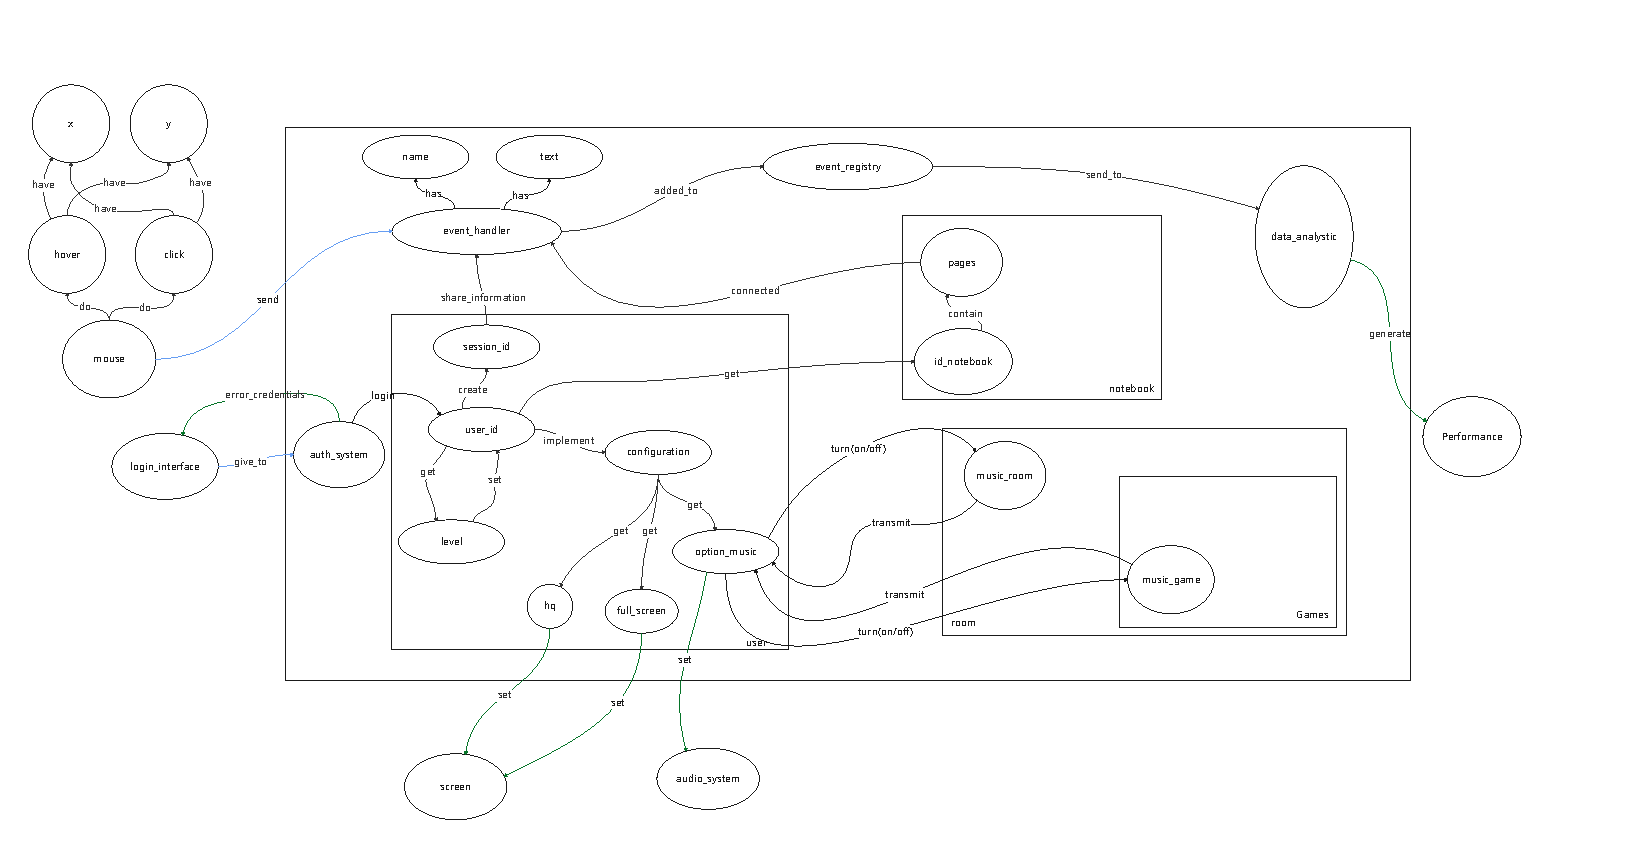
\includegraphics[width=0.75\textwidth]{src/IO.pdf}
  \end{center}

  \section*{Complexity and Sensitivity}
  Sensitivity analysis allows us to understand how changes in one component of the system can affect the entire system. To do this, we analyze how each component influences the system and to what extent, with a particular focus on those components where sensitivity is highest—i.e., where variations in the output can most significantly impact the overall system. All of this is aimed at predicting player performance based on how these components behave.\\
  
  \textbf{First, we begin with the inputs. In the system, two inputs were defined.}
  
  \subsection*{Login Interface – Auth Login}
  The login interface is the user's entry point to access the game, and the auth login is the component that determines whether the user is allowed in or not. Although they do not directly affect the system, these elements are what enable the user to interact with the game itself.
  
  \subsection*{Mouse Events}
  Events refer to the actions performed by the player using the mouse. These actions have a significant impact on the system, as depending on the decisions the player makes, how they make them, and the time taken to execute them, the system will respond in different ways. While there is not complete randomness—since in games actions are predefined—the variation lies in how the player carries them out.
  \\
  
  \textbf{Now that we have analyzed the inputs, we will analyze the system components that influence the system.}
  
  \subsection*{Level}
  The level reached by the player is a key element, as it reflects the progress and skills acquired during the game. However, it may present some limitations depending on the context, since this factor also largely depends on the player's ability, whether or not they use cheats to advance, and so on.
  
  \subsection*{Session Id}
  The duration of each session per player allows for the analysis of whether players quickly become engaged with the game or, on the contrary, abandon it quickly. This factor is important for predicting player performance.
  
  \subsection*{Configuration}
  Configuration is a very important aspect, as it can significantly influence the player's performance. Depending on the settings the player has adjusted, their in-game performance may vary in different ways. For the system presented, these settings include music volume, whether the game is in fullscreen mode, and the game’s quality.
  
  \subsection*{Data Analytics}
  This system component will analyze the outputs of the previously described components to identify patterns that help determine player performance. The limitations of this component are directly related to the inputs—therefore, if these are biased, the prediction will be as well.
  


  \section*{Conclusion}
  The system, based on the analysis performed, demonstrates a certain robustness in its relationships. This property ensures that its results are more precise and less susceptible to errors.\\
  Although some uncertainty remains, it revolves around understanding the type of games it offers does the catalog exhibit a high and significant level of skill? These questions are necessary 
  to provide a clearer understanding of the variability in configurations \\
  We observe that the impact of each element is balanced in relation to both the system and its objective. 
  While one component stands out such as \underline{\textbf{event\_handler}} and 
  \underline{\textbf{event\_registry}} we can still note an overall balance in the importance weights.\\
  Another important point is its internal configuration. Here, we can identify small subregions that improve diagram readability regions with significantly strong influence that,
   in addition to providing balance (as previously mentioned), offer control over the problem's surface and its purpose.

\end{document}
